\chapter{Testovanie a evaluácia}
\label{kap:tes}

MEŠKANIE
V tejto ukážke môžeme pozorovať ako sa zmenila vyhľadaná cesta v závislosti od meškania. 
Hľadáme cestu s vyhľadávacími parametrami na obrázku (a). Najskôr algoritmus hľadal len nad statickými cestovnými poriadkami. Našiel preto jednu najrýchlejšiu cestu na obrázku (b). 
Po tom ako sme v algoritme začali prihliadať na meškanie vozidiel, zmenil sa aj výsledok vyhľadávania (obrázok ©). 
Na obrázku (e) je riadok z dát o meškaní vozidiel, ktorý poukazuje na to, že v deň 5.2.2018 v čase 9:59 nadobudla linka 5 na zastávke Karlova Ves meškanie 1 minútu. Vyhľadávanie sme spustili 5.2.2018 v čase 10:00. Deň 5.2.2018 je v konfigurácii nastavený ako aktuálny dátum. 

Jazda linky 5 príde na zastávku Botanická záhrada s meškaním a z toho dôvodu sa mení aj prestupná zastávka. Čas na prestup na zastávke Vysoká, Tchibo Outlet by bol 0 minút a v parametroch je predvolený minimálny čas na prestup 1 minúta. Prestupnou zastávkou sa preto stala zastávka Poštová, MARTINUS.

Všimnime si ešte označenie meškania. Meškajúci spoj má zafarbené časy červenou farbou. Po kliknutí na detail (obrátok (d) ) vidíme, aj hodnotu meškania spoja. Časy z druhého spoja sú čiernou farbou, pretože tento spoj ešte nevyrazil zo začiatočnej zastávky v čase vyhľadávania (10:00).

\begin{figure}[H]
\centerline{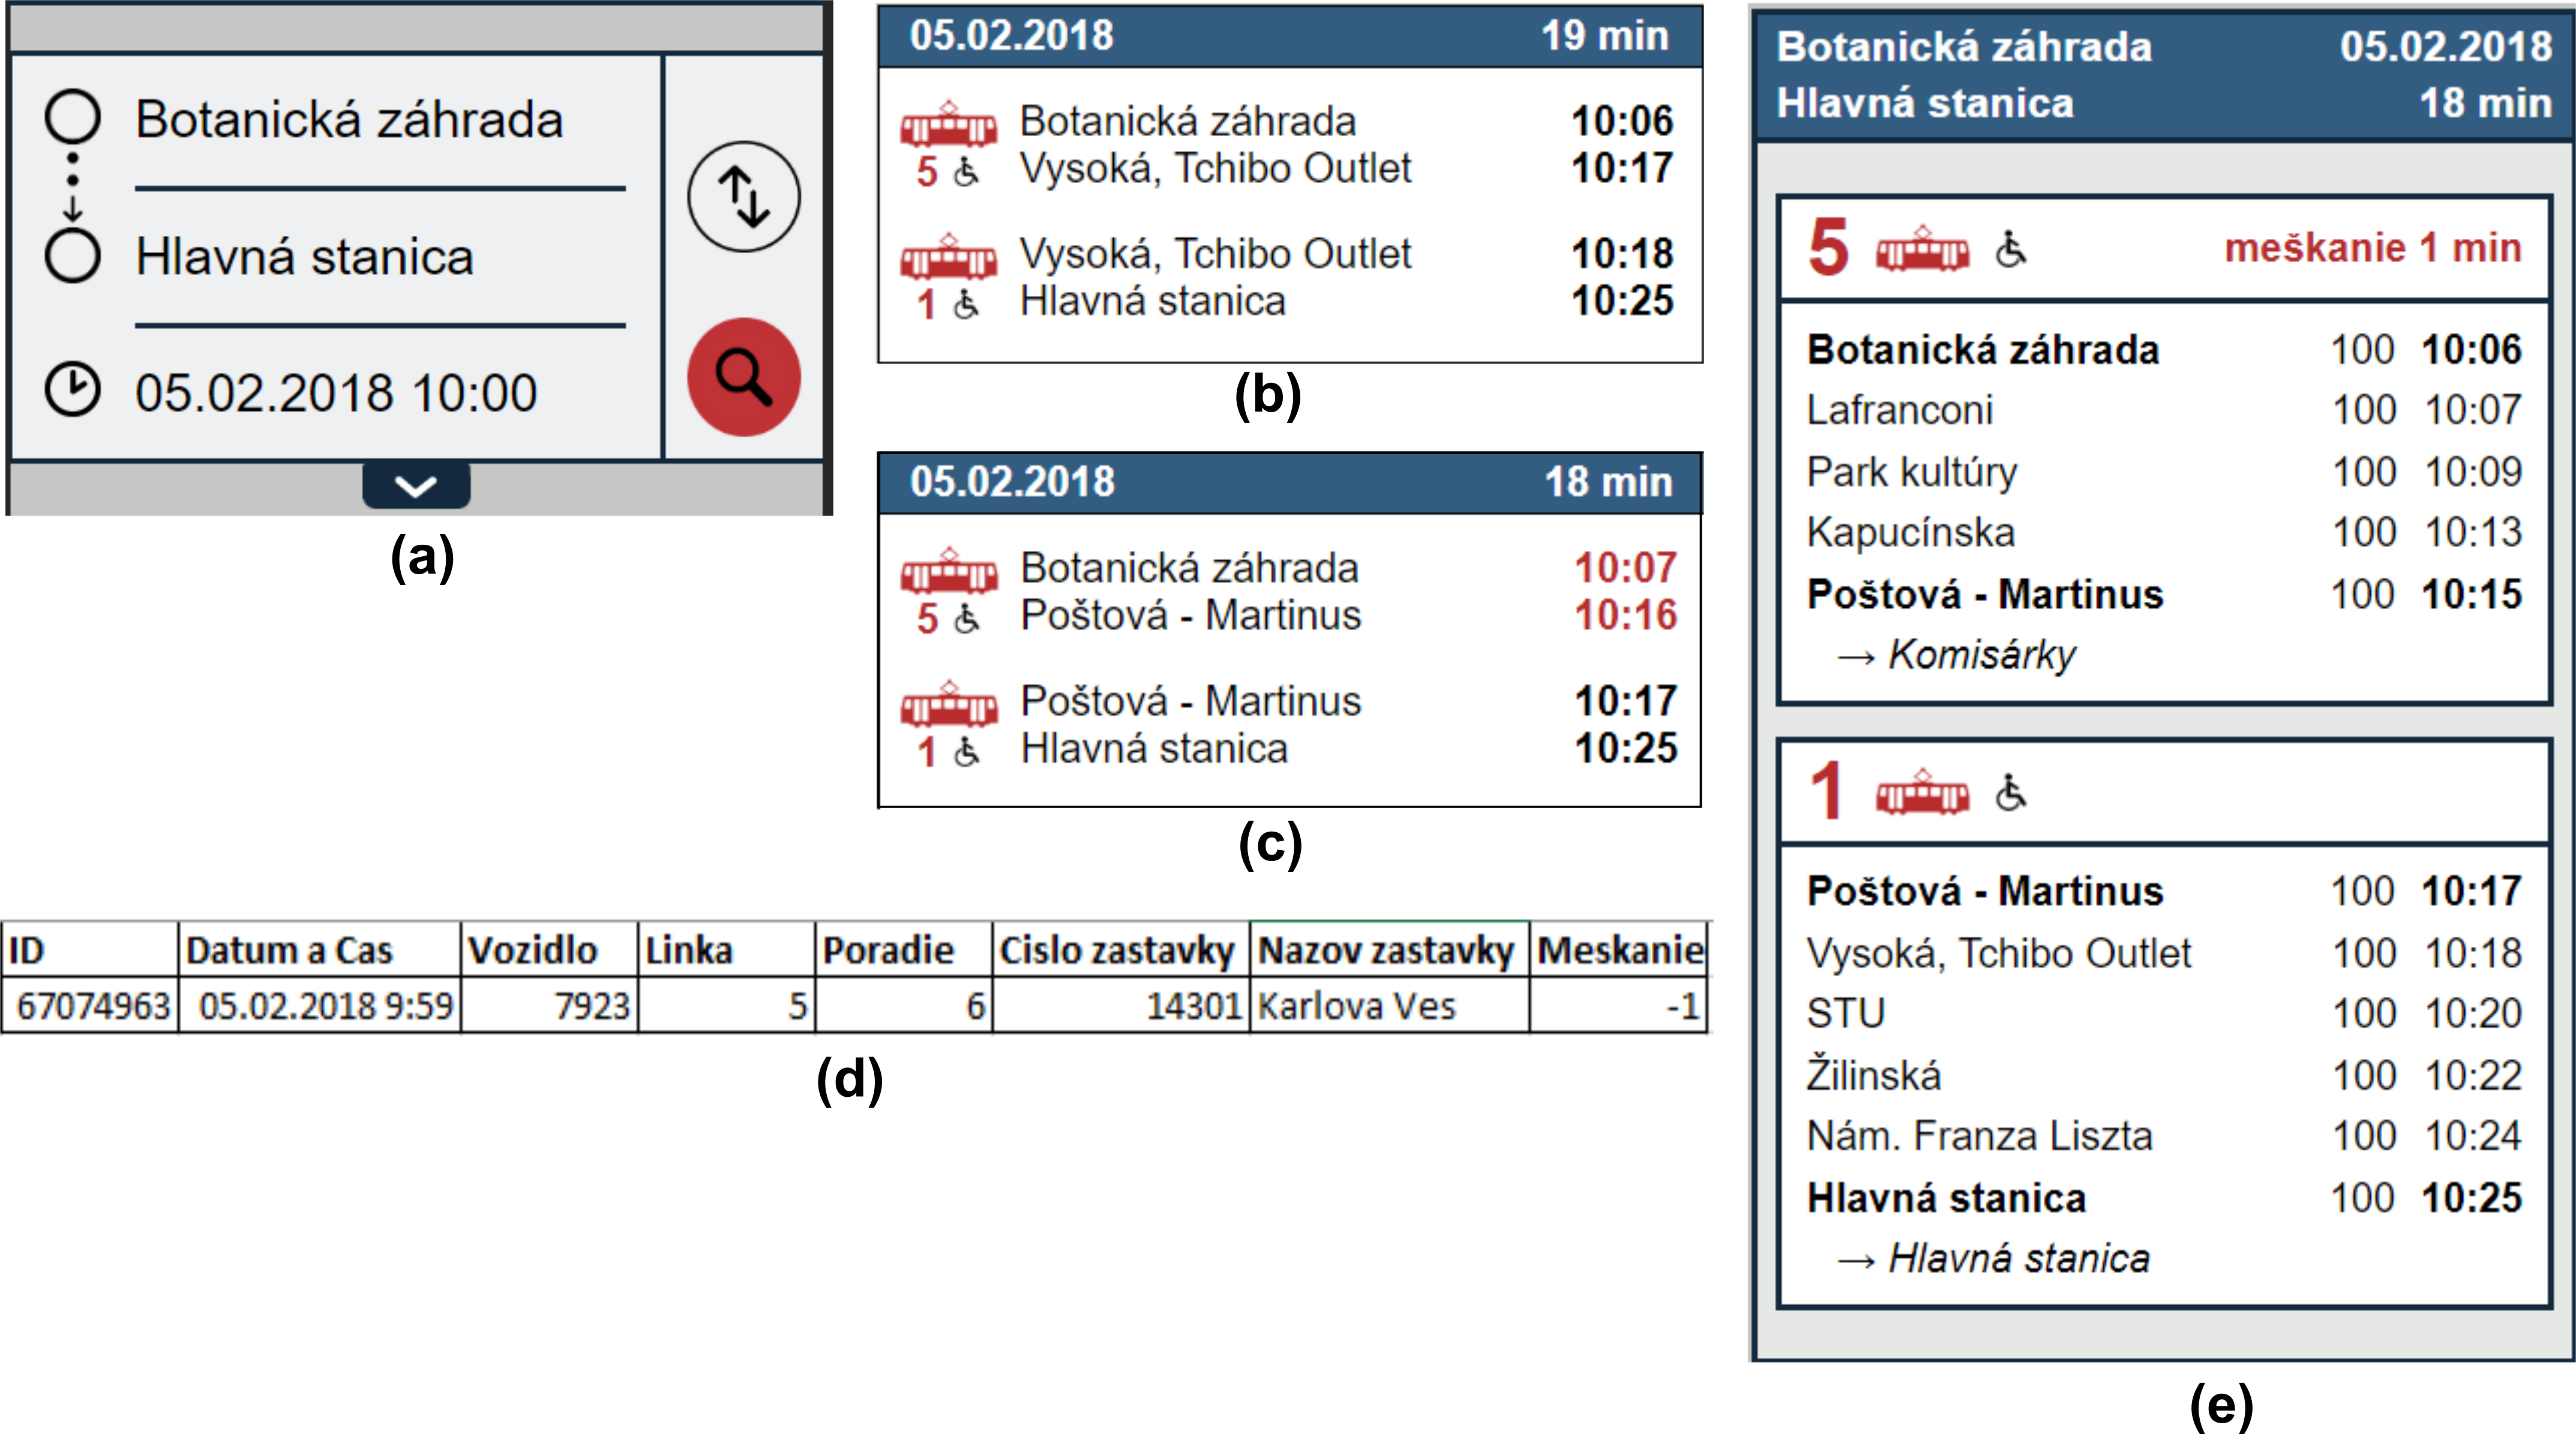
\includegraphics[width=1.0\textwidth]{images/test-delay1}}
\caption[Testovanie meškania]{Testovanie meškania}
\label{fig:test-delay}
\end{figure}

\begin{figure}[H]
\centerline{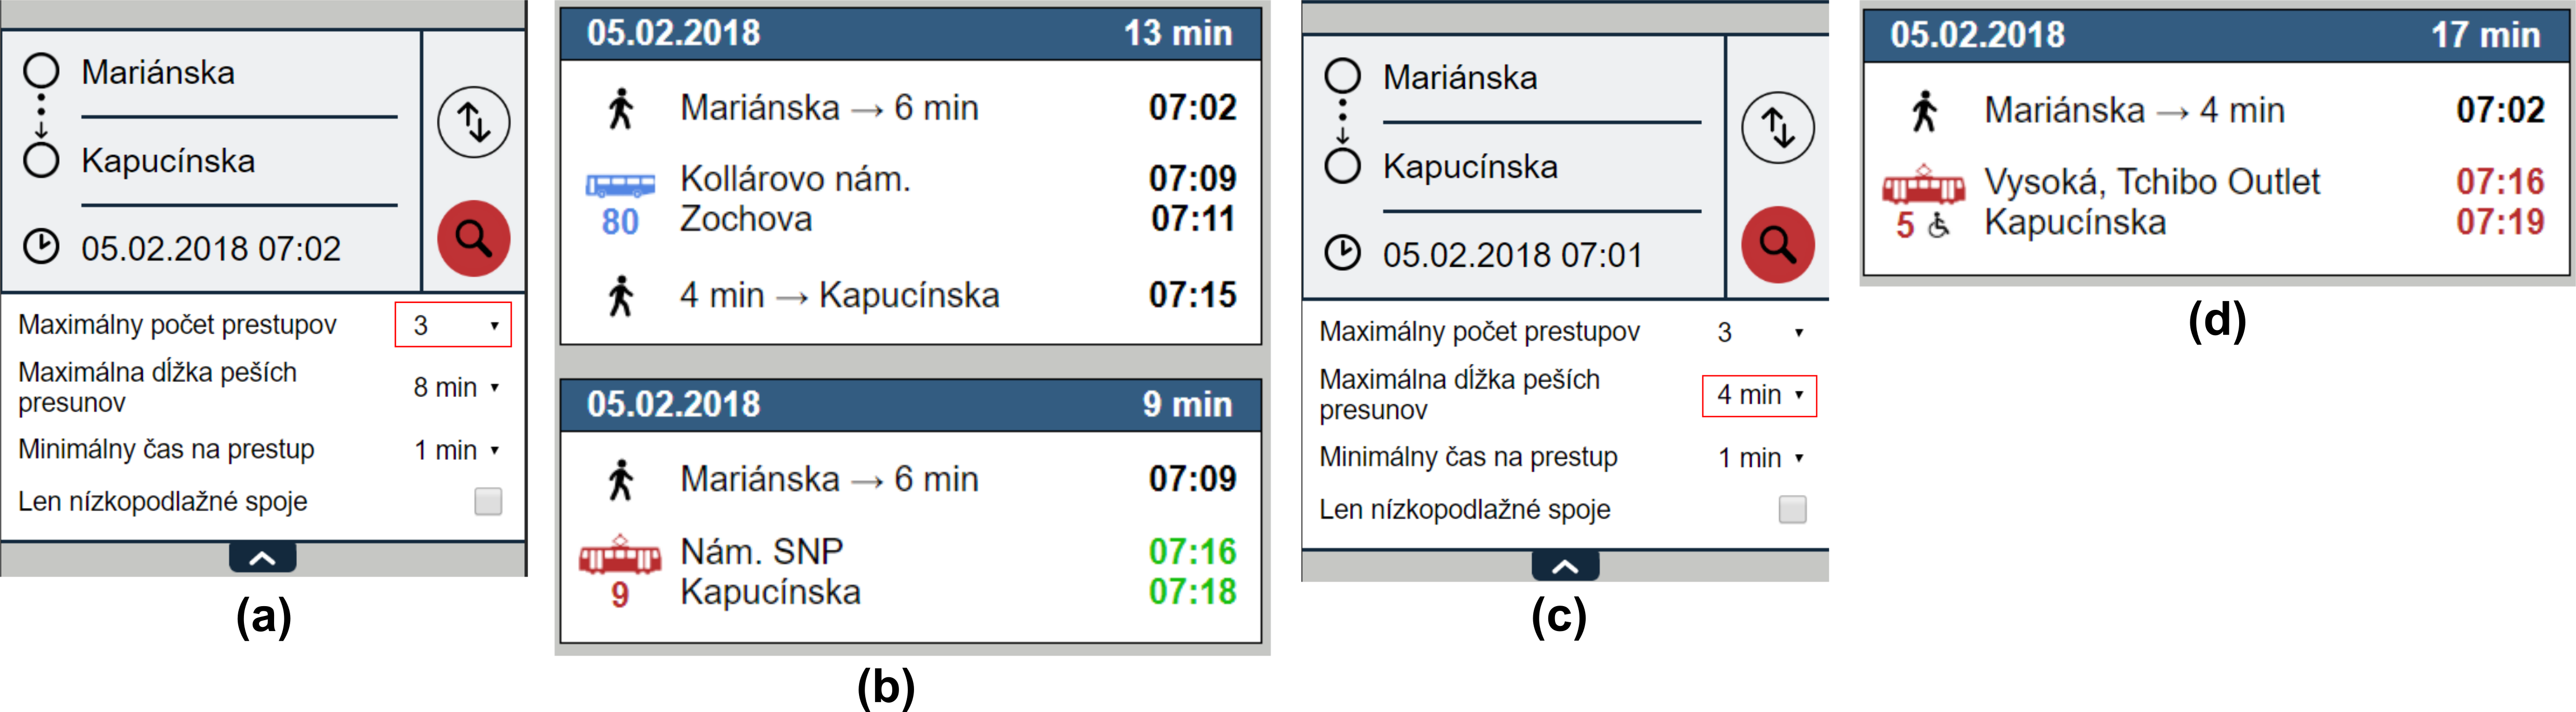
\includegraphics[width=1.0\textwidth]{images/mf-3}}
\caption[Testovanie meškania]{Testovanie meškania}
\label{fig:test-delay}
\end{figure}

